% by Wolfgang
\section{Introduction} 
Artificial intelligence (AI) is one of the most exiting topics in computer science for research as well as for the public of the current time. We have seen impressive results of learning machines doing all kinds of difficult tasks. And there is general excitement among AI advocates of this technology and the future this mind bring. Often these AI enthusiasts are criticized of glorifying machines, that can never act, decide and create on a human level, so the opinion of some critics. And in fact there are tasks that are beyond the capabilities of current AI approaches; where the goal is not clear and the direction towards it is not visible. In this situations where the machine fails a human can often easily spot the write move to do and even if not he can sometimes intuitively look for the answer in the write direction. This form of problem solving is based on creativity, a capability that is most often exclusively granted to humans. An other part of creativity is the generation of innovative ideas and goods. So what makes creativity and is it really exclusively present in biological machinesv that is the human. We think that in order to understand the human mind we have look at the thinks that makes it unique. We also believe that creativity can artificially be reproduced and studied. In this work we propose a method of procedural creativity and apply in to the music domain, by generating new music.

According to a popular theory of mind (Computational theory of mind) 
the human cognition is nothing more then a information processing machine. A complex and very efficient machine though, but a machine. Following this idea we ask the question whether the possibility to implement aspects of creativity in an AI exists and what would be needed to do so. We have chosen the music domain for that. We implemented a program that is able to create new music after it has heard other music.

\subsection{The Music Domain}
We have chosen the music domain for several reasons. First it is an area that enables creativity, there is a whole culture around music creation and playing music. Even thou creativity can be applied in any area (think about the creative problem solving) we wanted to work in a domain that is only 'solvable' with creativity, that way we at least have to approximate creativity mechanisms to get a result.

Second music has a representation on many different levels, similar to what we in human cognition. On the basic layer sound are moving particles in a wave of high and low air pressure, that get interpreted as movements in the inner ear. If the air wave is constant we talk about tones. Music deals with tones on a scale. Starting at one root tone in music theory the tonality is build in a hierarchical fashion of intervals, i.d frequencies of the sound wave. At this layer of tone representation we normally start talking about music. It is clear that we already make some assumptions on how we perceive sound and what might sound good. Normally in western music we just consider the Dur tonalities, and we will do so in this work. 

The next layer are tones in the tonality ordered to a sequence. This layer describes what tones are played after another and what tones are played at the same time, in the music domain we normally talk of melody and harmony. We choose to work on this layer of symbolic representation. But there are even higher layers of music that are worth considering. There are different pieces of music and whole concerts with each a theme or a story and artists have different styles. This higher levels of music make use of non music concepts such as stories and emotions. 

The interesting part about this is that all of these layers also are processed in a different way by humans. While creating (or just listening to) music all these layers are combined. But also the single layers are subject of inspection and one can be creative and inventive there as well. These properties are very useful for our exploration in computational creativity. This way we can focus on specific layers of the creative process and consider similar layers in the human cognition. By that we are able to build cognitive inspired models that can also be discussed on the basis of information processing in the human brain. 

\subsection{The Project Approach}
The main idea of the project is to build the computer program to test procedural creativity methods that are able to produce music on its own 

To explore the methods we built a framework to test and explore computational accounts for music harmonization. This section will introduce this framework, later we will refer to the parts in more detail.

While designing the framework the guiding principles were molecularity and simplicity. The pipeline from input to output consisted of: Music representation - music piece (melody) - develop style - apply style to melody / harmonization - output music (e.g. musicxml)

Important to notice here is the differentiation between the 'creative' part and the harmonization part. We follow a two step process that consists of a style generation (creative) and the harmonization where this style is applied to the melody (deterministic). This way we can explore different 'creative' modules in our abstract representation and then have the same predictive harmonization process in the end, to project it back into music space.

\subsection{System Architecture}
The system's pipeline is visualized in Figure \ref{fig:arch}. The left side shows the input to the system, that consists of a melody to harmonize and a couple of known styles. All music that is input to the system is represented using our music representation using a sequence of vectors.
\begin{figure}
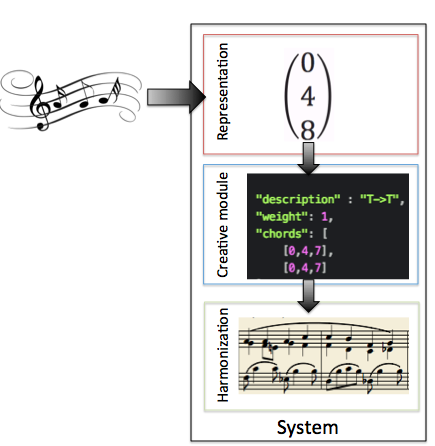
\includegraphics[scale=1]{Chapters/pic/sys_arch.png}
\caption{The architecture of the system}
\label{fig:arch}
\end{figure}


These styles are given by the user or generated out of other music or are the result of earlier runs and outcomes of the system.

The first part of the two step process is the creative part. Here the system creates a new style with given styles. This is where the creative algorithms are located. The user can choose one of the creative modules and different styles to create different new styles. In the next step the new style is then used as a template to harmonize the given melody. This step is not considered creative but made to be very predictive.

By splitting the process we are able to test different creative modules and produce just the style. We can then either just visualize the style as the essence of the creative module or run the deterministic harmonization process with a melody to be able to listen to the creation. 